\documentclass[a4paper, parskip=half, 11pt]{scrartcl}

\usepackage{submarinerules}
\usepackage[margin=1.5cm]{geometry}
\usepackage{multicol}
\setlength\columnsep{1.0cm}

\begin{document}
\pagestyle{empty}

\begin{center}
\begin{tikzpicture}
\clip (-\textwidth/2, 0.5in) -- (\textwidth/2, 0.5in) -- (\textwidth/2, -0.5in) -- (-\textwidth/2, -0.5in) -- cycle;

\node[fill=Blue, inner sep=0.4cm, minimum width=\textwidth] at (0,0) {\setmainfont[Scale=3.0]{Chakra Petch-Bold}\Huge \textcolor{Goldenrod}{PING}};

\node[circle, minimum width=2.0in, fill=Goldenrod, opacity=1, inner sep=0pt] at (-2.375in, 0) {};
\node[circle, minimum width=1.75in, fill=Blue] at (-2.375in, 0) {};
\node[circle, minimum width=1.5in, fill=Goldenrod, opacity=1] at (-2.375in, 0) {};
\node[circle, minimum width=1.25in, fill=Blue] at (-2.375in, 0) {};
\node[circle, minimum width=1.0in, fill=Goldenrod, opacity=1] at (-2.375in, 0) {};
\node[circle, minimum width=0.75in, fill=Blue] at (-2.375in, 0) {};
\node[circle, minimum width=0.5in, fill=Goldenrod, opacity=1] at (-2.375in, 0) {};
\node[circle, minimum width=0.25in, fill=Blue] at (-2.375in, 0) {};

\node[circle, minimum width=2.0in, fill=Goldenrod, opacity=1] at (2.375in, 0) {};
\node[circle, minimum width=1.75in, fill=Blue] at (2.375in, 0) {};
\node[circle, minimum width=1.5in, fill=Goldenrod, opacity=1] at (2.375in, 0) {};
\node[circle, minimum width=1.25in, fill=Blue] at (2.375in, 0) {};
\node[circle, minimum width=1.0in, fill=Goldenrod] at (2.375in, 0) {};
\node[circle, minimum width=0.75in, fill=Blue] at (2.375in, 0) {};
\node[circle, minimum width=0.5in, fill=Goldenrod] at (2.375in, 0) {};
\node[circle, minimum width=0.25in, fill=Blue] at (2.375in, 0) {};

\node at (-2.375in, 0) {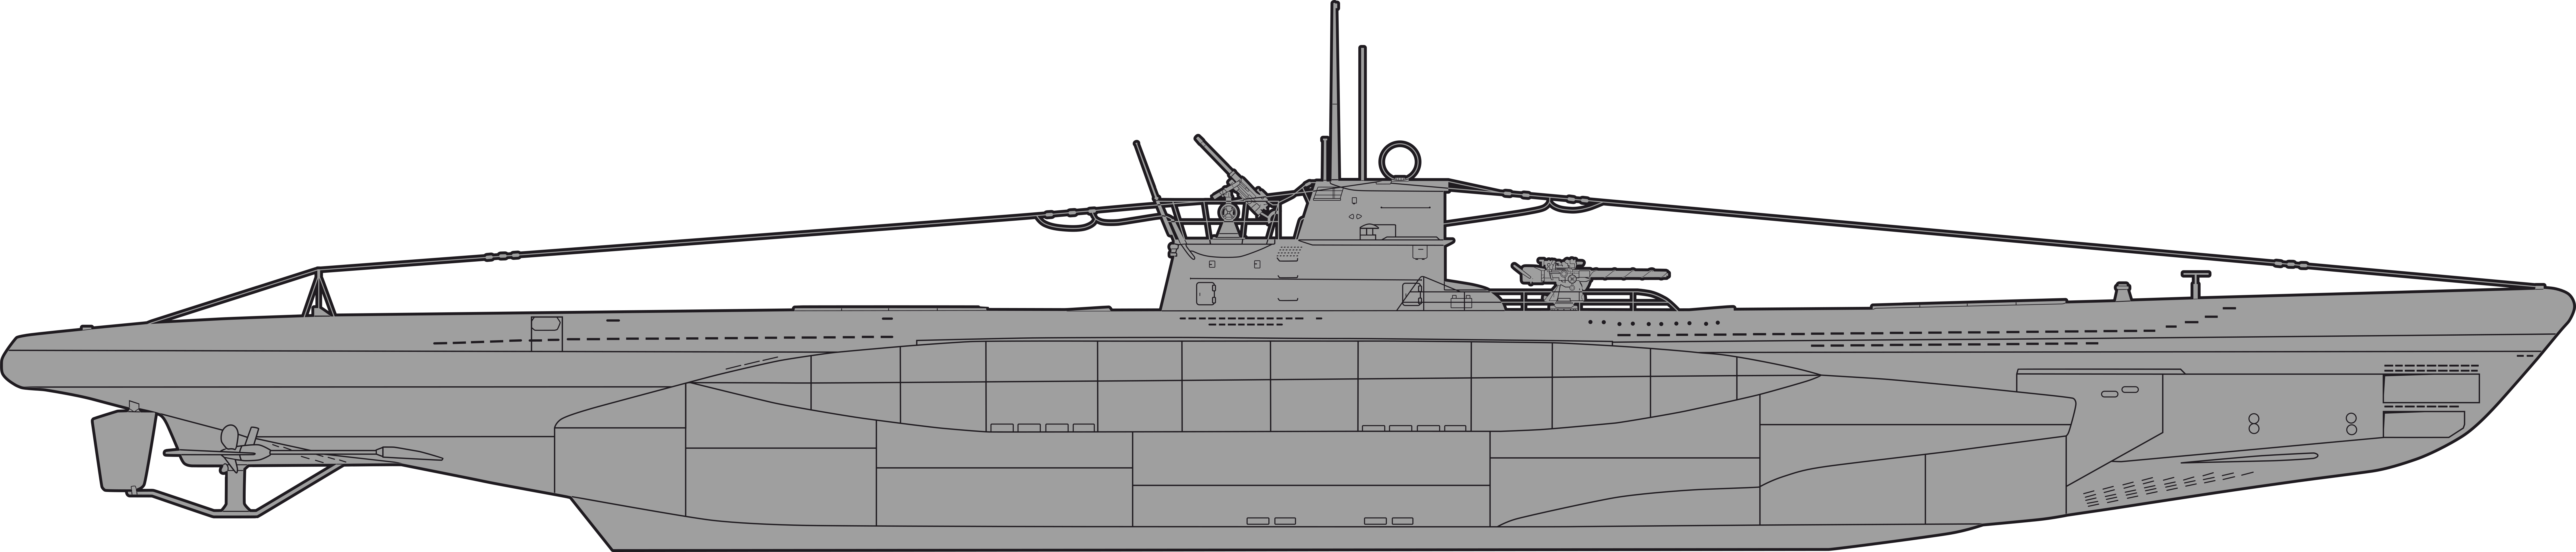
\includegraphics[height=0.425in]{uboat_dark.png}};
\node[xscale=-1] at (2.375in, 0) {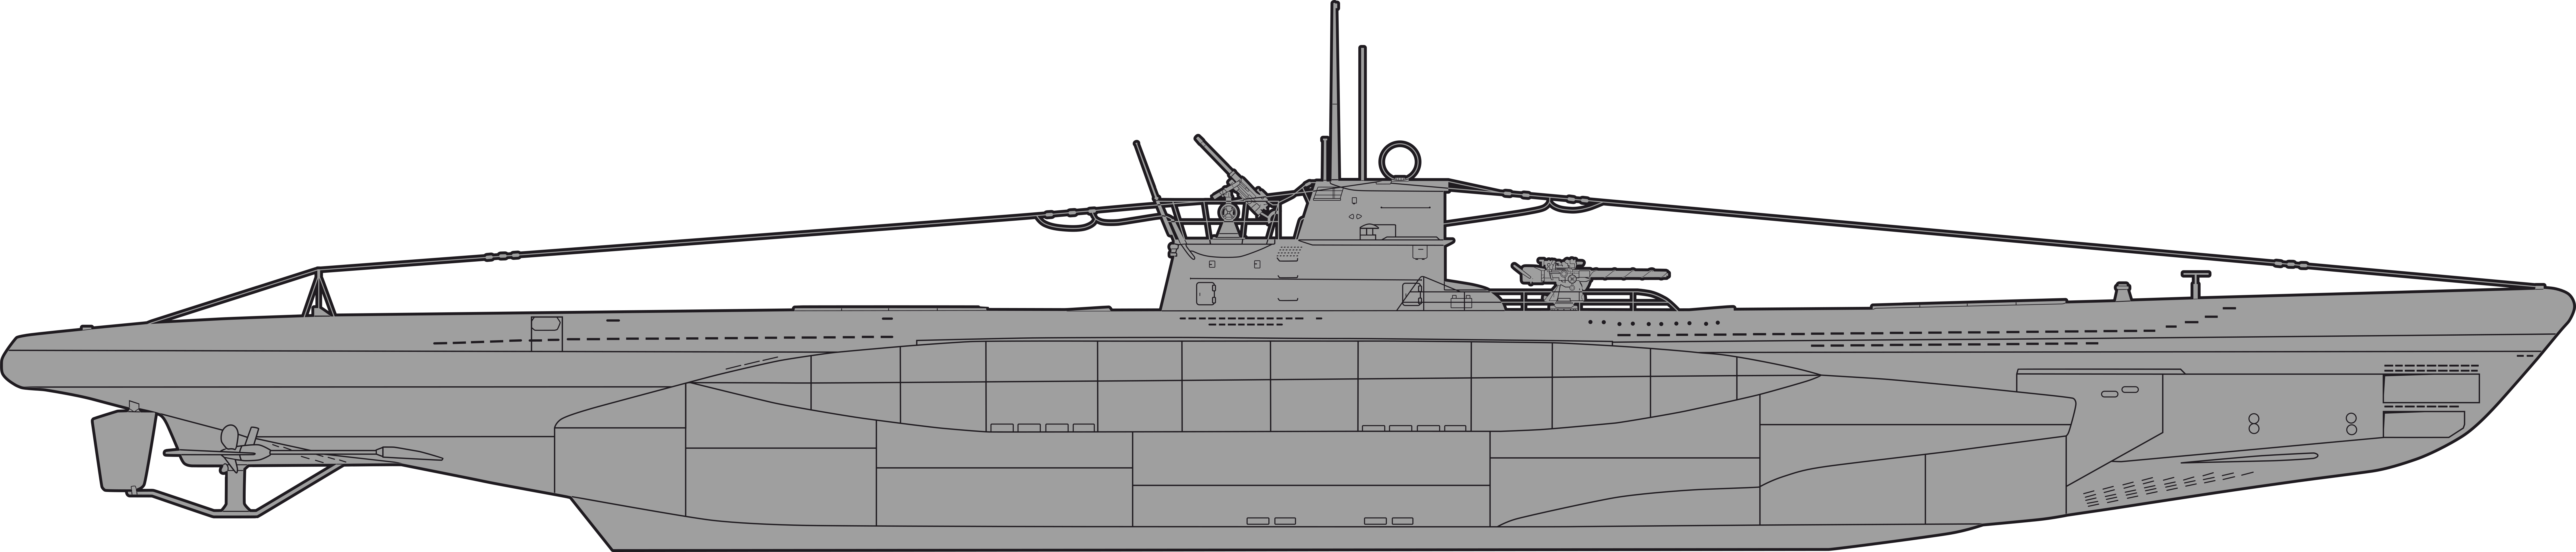
\includegraphics[height=0.425in]{uboat_dark.png}};
\end{tikzpicture}
\end{center}

\vspace{0.8ex}

\begin{multicols}{2}
\section*{Overview}
\PING{} is a tactical hidden-movement game where the cards you play can come back to sink you. You and your adversary will assume the roles of rival submarine captains who are locked in a deadly duel in the deep.

Be the first to complete five strategic objectives or to sink your adversary's submarine.

\PING{} is a game for two players and can be played in approximately twenty minutes.


\section*{Components}
%\PING{} is played with a deck of eighteen cards.
\vspace{1ex}
\begin{center}
\begin{minipage}{0.45\linewidth}
\begin{center}
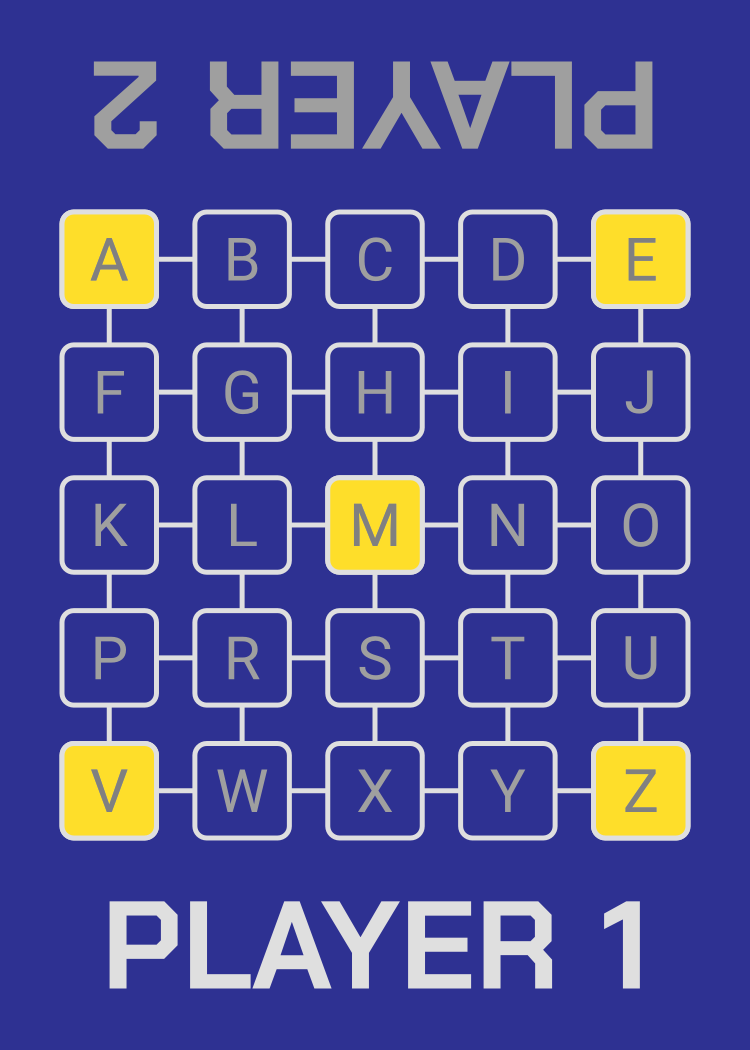
\includegraphics[height=3.5cm]{location_card.png}
\vspace{1.5ex}

2 location cards
\end{center}
\end{minipage}
\begin{minipage}{0.45\linewidth}
\begin{center}
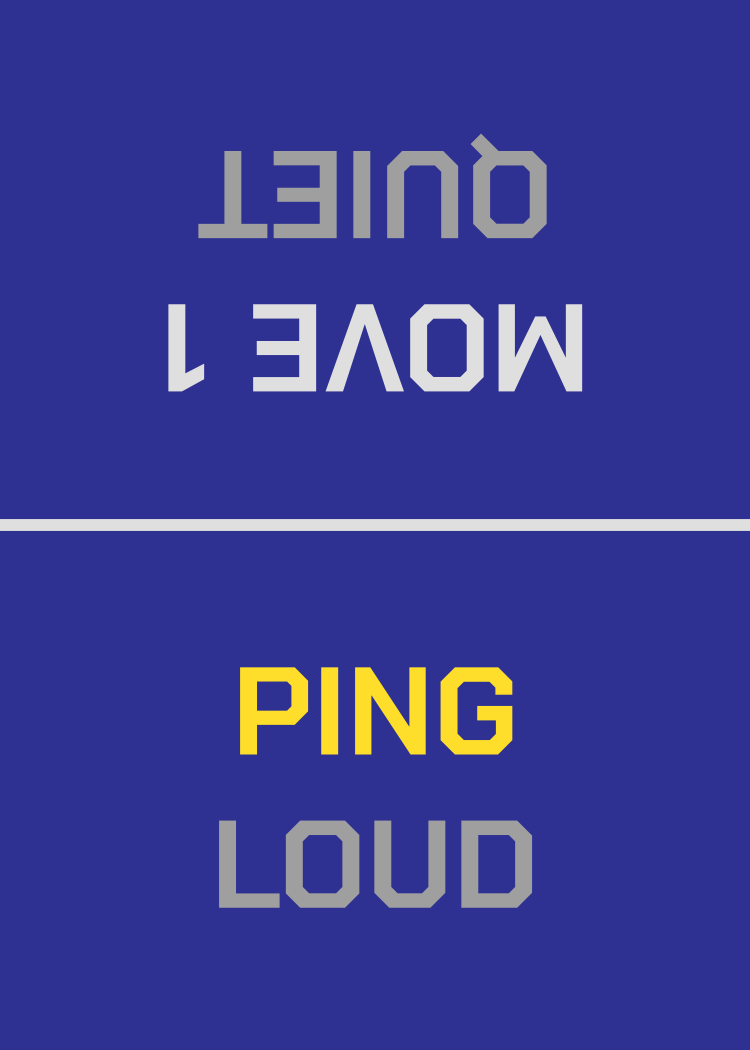
\includegraphics[height=3.5cm]{action_card.png}
\vspace{1.5ex}

16 action cards
\end{center}
\end{minipage}
\end{center}

%\begin{figure}[h] \centering
%    \begin{subfigure}[b]{0.45\textwidth}
%    		\centering
%        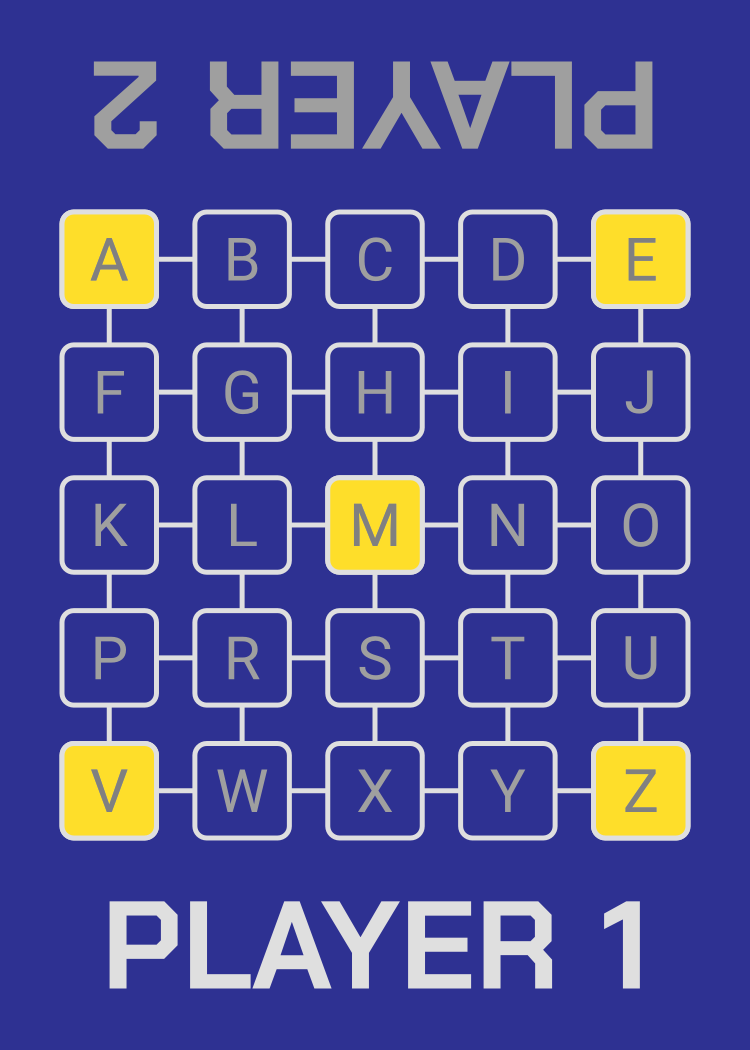
\includegraphics[height=3.5cm]{location_card.png}
%        \caption*{2 location cards}
%        \label{fig:a}
%    \end{subfigure}
%    \begin{subfigure}[b]{0.45\textwidth}
%    \centering    
%        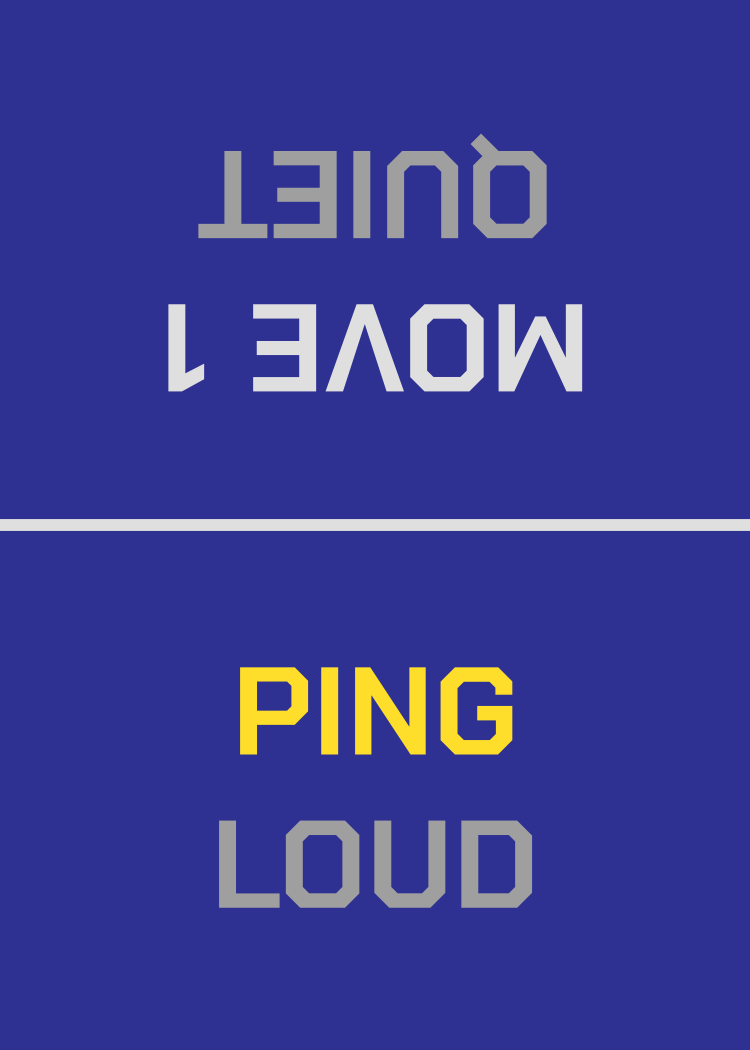
\includegraphics[height=3.5cm]{action_card.png}
%        \caption*{16 action cards}
%        \label{fig:b}    
%    \end{subfigure} 
%\end{figure}


\vspace{1ex}
\section*{Set Up}
\begin{enumerate}[leftmargin=*]
	\item Sit across the table from your adversary with the play area between you.
	\item Give each player a location card. 
	\item Shuffle the deck of sixteen action cards.
	\item Deal three action cards to each player.
	\item Place one action card face down in the play area. Place it on the right-hand side of the play area as viewed by Player 1.
	\item Set the remaining nine action cards aside. You will not use these cards during the game.
	\item Secretly choose your starting location. You may start on any grid square. Use your location card to indicate your choice (see {\setmainfont{Chakra Petch}{\textcolor{Blue}{\textbf{TRACKING LOCATIONS}}}}).
\end{enumerate}


\vfill\null
\columnbreak


%\section*{Playing the Game}
Starting with Player 1, take turns playing action cards (see {\setmainfont{Chakra Petch}{\textcolor{Blue}{\textbf{ACTION CARDS}}}}). You win if you complete all five strategic objectives (see {\setmainfont{Chakra Petch}{\textcolor{Blue}{\textbf{STRATEGIC OBJECTIVES}}}}) or if you sink your adversary's submarine (see {\setmainfont{Chakra Petch}{\textcolor{Blue}{\textbf{DAMAGE AND REPAIR}}}}).
%\begin{itemize}[leftmargin=*]
%\item Complete all five strategic objectives\\(see {\setmainfont{Chakra Petch}{\textcolor{Blue}{\textbf{STRATEGIC OBJECTIVES}}}}).
%\item Sink your adversary's submarine\\(see {\setmainfont{Chakra Petch}{\textcolor{Blue}{\textbf{DAMAGE AND REPAIR}}}}).
%\end{itemize}

\section*{Tracking Locations}
During the game, you will use your location card to track your submarine's location on a \emph{grid}. 

To do so, gently pinch your location card between your thumb and middle finger such that your thumb is touching your submarine's current location.
As you move, adjust your grip on your location card accordingly.

Two grid squares are \emph{adjacent} only if there is a line connecting them (no diagonals).

\textit{\textbf{Pro Tip:} Keep your location card hidden. If your adversary can see your location card, it will be much easier for them to target you.}


\section*{Action Cards}
Starting with Player 1, take turns playing action cards.
Each action card can be played to perform either a \emph{movement action} or a \emph{utility action}.

When you play an action card, place it on the left-hand side (from your perspective) of the play area with the action you are using it to perform closest to the center of the play area.

If the action name is written in yellow, play the card face up. Otherwise, play it face down.

Some actions have \emph{tags}, e.g.  \LOUD{} and \QUIET{}, that affect their behavior. In particular, you must reveal your location after you take any \LOUD{} action.

After you play an action card, perform the action described thereon.
Then, add the action card on the right-hand side (from your perspective) of the play area to your hand.


\subsection*{Movement Actions}
When you perform a movement action you will take a specified number of \emph{steps} by moving from your current location to an adjacent grid square.  Because it is \LOUD{}, you must reveal your location when you take the \MMMOVE{} action.
%\begin{description}[leftmargin=1em, labelwidth=0pt, labelsep=0pt]
%\item[]\MOVE{} (\QUIET{})\ \ Take 1 step.
%\item[]\MMOVE{}\ \ Take 2 steps.
%\item[]\MMMOVE{} (\LOUD{})\ \ Take 3 steps. Reveal your location.
%\end{description}

\vfill\null

\end{multicols}

\vfill

\hrulefill

{\textbf{Design}: Michael Purcell \hfill \makeatletter\textbf{Version:} \@version\makeatother \hfill \textbf{Contact}:~\href{mailto:mike@armiger.games}{mike@armiger.games}}

\newpage

\begin{multicols}{2}


\subsection*{Utility Actions}
\begin{description}[leftmargin=1em, labelwidth=0pt, labelsep=0pt]
\item[]\PPING{} (\LOUD{})\ \ Reveal your location. Turn your adversary's previous action card face up. If it is not \DEEP{}, they must reveal their location.
\item[] \LISTEN{} (\QUIET{})\ \ Turn your adversary's previous action card face up. If it not \DEEP{} or \QUIET{}, they must reveal their location.
\item[]\LAUNCH{} (\LOUD{})\ \ Reveal your location. Pick a direction in which to launch a torpedo. If it passes through your adversary's location, they take damage (see {\setmainfont{Chakra Petch}{\textcolor{Blue}{\textbf{DAMAGE AND REPAIR}}}}). You may not target your own location.
\item[]\SHOOT{} (\LOUD{})\ \  Reveal your location. If your adversary is in the same location as you or if they are in a location adjacent to yours, they take damage (see {\setmainfont{Chakra Petch}{\textcolor{Blue}{\textbf{DAMAGE AND REPAIR}}}}).
\item[]\ENCRYPT{}\ \ Complete a strategic objective at your location. Do not reveal your location.
\item[]\DIVE{} (\DEEP{})\ \  Do nothing on this turn. If your adversary takes the \LAUNCH{} or \SHOOT{} action on their next turn, turn this action card face up to nullify their action.
\end{description}



\section*{Example}
Player 2 (top) took the \PPING{} action on their turn.
Because the action name is written is yellow, they played their action card face up.

\vspace{-1ex}

\begin{center}
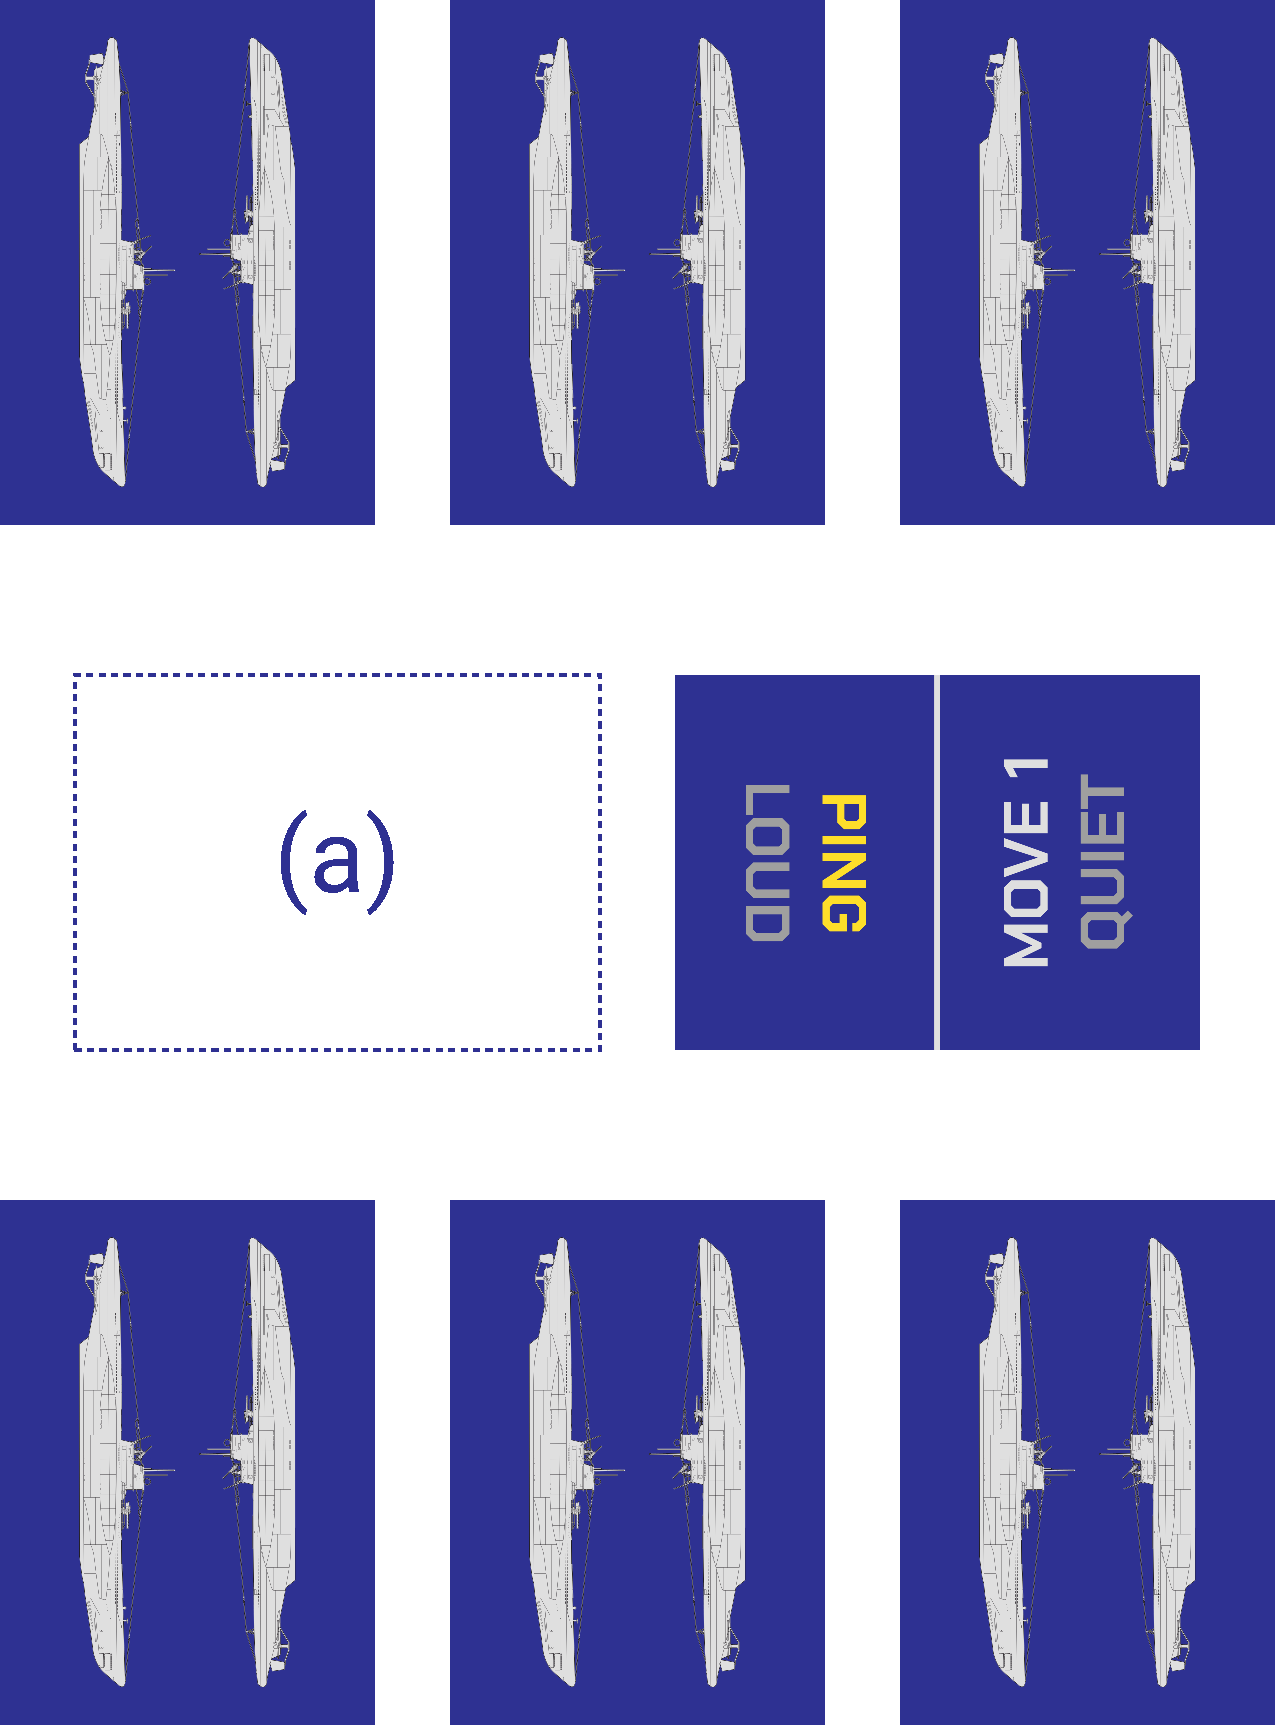
\includegraphics[width=0.5\linewidth]{example_diagram.pdf}
\end{center}

\vspace{-1ex}

Next, Player 1 (bottom) will take an action. They will place the corresponding action card in the play area (a).
Then, they will add the card on the right-hand side of the play area to their hand.


\vfill\null
\columnbreak

\section*{Strategic Objectives}
There are five locations, \sansA{} \sansE{} \sansM{} \sansV{} \sansZ{}, where you will be able to complete strategic objectives by sending a report back to fleet command.

When at one of these locations, you may either:
\begin{itemize}[leftmargin=*]
	\item Send an unencrypted report. Reveal your location to complete the strategic objective at your location. This can be done at any point during your turn and does not require you to spend an action to do so.
	\item Send an encrypted report. To do so, take the \ENCRYPT{} action (see {\setmainfont{Chakra Petch}{\textcolor{Blue}{\textbf{UTILITY ACTIONS}}}}) on your turn to complete the strategic objective at your location.
\end{itemize}

You may only complete the strategic objective at each location once per game.

\textit{\textbf{Pro Tip:} Wait to send an unencrypted report until just before you play an action card.}



\section*{Damage and Repair}
%If your adversary takes the \LAUNCH{} or \SHOOT{} action, you may \emph{take damage}. 

When you take damage, your adversary will select two action cards in your hand to \emph{disable}.
Turn these cards sideways to indicate that they have been disabled.
Then, reveal your location.

%Action cards that have been disabled cannot be played in the usual fashion.
When you play a card that has been disabled, you may not take an action.
Instead, you are \emph{repairing} your submarine.

After playing an action card that has been disabled, add the card on the right-hand side of the play area to your hand as normal.
%So, repairing damage to your submarine reduces the number of disabled cards in your hand by one.

If all three of the action cards in your hand are disabled, then your submarine sinks. The game ends immediately and your adversary wins.

\textit{\textbf{Pro Tip:} Shuffle the action cards in your hand before your adversary selects which will be disabled when you take damage.}


\section*{End of Game}
You win immediately if you complete all five strategic objectives or if you sink your adversary's submarine. 


\vfill\null

\end{multicols}

\vfill

\hrulefill

{\textbf{Design}: Michael Purcell \hfill \makeatletter\textbf{Version:} \@version\makeatother \hfill \textbf{Contact}:~\href{mailto:mike@armiger.games}{mike@armiger.games}}

\end{document}
